\documentclass[12pt,a4paper,twoside]{book}
\usepackage{amsmath}
\usepackage{setspace}
\usepackage{geometry}
\usepackage{times}
\usepackage{fancyhdr}
\usepackage[utf8x]{inputenc}
\usepackage{graphicx}
\usepackage{xcolor}
\usepackage{listings}
\graphicspath{ {immagini/} }
\fancyhf{} % clear all header and footers
\renewcommand{\headrulewidth}{0pt} % remove the header rule
\fancyfoot[LE,RO]{\thepage} % Left side on Even pages; Right side on Odd pages
\pagestyle{fancy}
\fancypagestyle{plain}{%
  \fancyhf{}%
  \renewcommand{\headrulewidth}{0pt}%
  \fancyhf[lef,rof]{\thepage}%
}

\usepackage{pdfpages}
\usepackage[italian,english]{babel}
\usepackage[hyphens,spaces,obeyspaces]{url}
\usepackage[hidelinks]{hyperref}
\usepackage[T1]{fontenc}

\usepackage{float}

\usepackage{titlesec}
\titleformat{\chapter}[hang] 
{\normalfont\huge\bfseries}{\chaptertitlename\ \thechapter:}{1em}{} 
\renewcommand{\chaptername}{Capitolo}

\colorlet{punct}{red!60!black}
\definecolor{background}{HTML}{EEEEEE}
\definecolor{delim}{RGB}{20,105,176}
\colorlet{numb}{magenta!60!black}
\lstdefinelanguage{json}{
	basicstyle=\normalfont\ttfamily,
	numbers=left,
	numberstyle=\scriptsize,
	stepnumber=1,
	numbersep=8pt,
	showstringspaces=false,
	breaklines=true,
	frame=lines,
	backgroundcolor=\color{background},
	literate=
	*{0}{{{\color{numb}0}}}{1}
	{1}{{{\color{numb}1}}}{1}
	{2}{{{\color{numb}2}}}{1}
	{3}{{{\color{numb}3}}}{1}
	{4}{{{\color{numb}4}}}{1}
	{5}{{{\color{numb}5}}}{1}
	{6}{{{\color{numb}6}}}{1}
	{7}{{{\color{numb}7}}}{1}
	{8}{{{\color{numb}8}}}{1}
	{9}{{{\color{numb}9}}}{1}
	{:}{{{\color{punct}{:}}}}{1}
	{,}{{{\color{punct}{,}}}}{1}
	{\{}{{{\color{delim}{\{}}}}{1}
	{\}}{{{\color{delim}{\}}}}}{1}
	{[}{{{\color{delim}{[}}}}{1}
	{]}{{{\color{delim}{]}}}}{1},
}



\geometry{a4paper,top=3cm,bottom=3cm,left=3cm,right=3cm,heightrounded,bindingoffset=5mm}
\onehalfspacing
\title{Documento merging di policy}
\date{Work in progress}
\author{Gianluca Oldani}

\begin{document}
\chapter{ODRL}
\section{Il linguaggio}
\subsection{Definizione ed obiettivi}
``L' Open Digital Rights Language (ODRL) è un linguaggio per l'espressione di policy che definisce: un modello dell'informazione flessibile ed interoperativo, un vocabolario e un meccanismo di codifica per la rappresentazione delle istruzioni sull'uso di contenuti o servizi''\cite{ODRLinfMod}.\\
Il linguaggio si pone all'interno dello scenario applicativo nel quale vi è la necessità di definire:
\begin{itemize}
	\item quali azioni siano permesse o proibite su una risorsa. Queste regole possono essere imposte da leggi o direttamente dal possessore dell'asset o servizio;
	\item indicare quali attori interagiscono con le policy definite; in particolare chi può definire le policy e a chi si applicano;
	\item indicare eventuali limiti riguardanti i permessi ed i divieti espressi;.
\end{itemize}
Avere un modello standard per definire questi bisogni dà 2 fondamentali vantaggi:
\begin{itemize}
	\item chi possiede l'asset è in grado di definire in modo chiaro quali siano le azioni che un consumatore può fare, evitanto quindi usi indesiderati;
	\item chi usufruisce dell'asset conosce in modo preciso quali azioni può compiere, evitando così di infrangere regole o leggi.
\end{itemize}
ODRL definisce un modello semantico di permessi, divieti ed obblighi, che può essere usato per descrivere le modalità d'uso di un contenuto. In particolare si cerca di definire i concetti chiave per la creazione di policy machine-readable collegate direttamente all'asset al quale sono associate, permettendo all'utente finale di reperire facilmente informazioni sulla risorsa che utilizza. Quest'ultimo requisito è soddisfatto, poiché ODRL è costruito seguendo i \textit{Linked Data principles}\cite{LinkedDataInfo}:
\begin{itemize}
\item Utilizzo di URIs come nomi per le risorse;
\item Gli URI sono indirizzi HTTP in modo che le persone possano cercare informazioni sulle risorse;
\item L'URI deve fornire informazioni utili sulla risorsa;
\item Tra le informazioni, fornire altri URI, in modo che l'utente possa raggiungere altre informazioni.
\end{itemize}
Nonostante questi principi siano più indicati per un'implementazione graph-based, è possibile anche definire utilizzi che non tengano conto dei link tra le varie informazioni.
\subsection{Il modello}\label{modello}
\begin{figure}[H]
	\centering
	\def\svgwidth{\columnwidth}
	\scalebox{0.5}{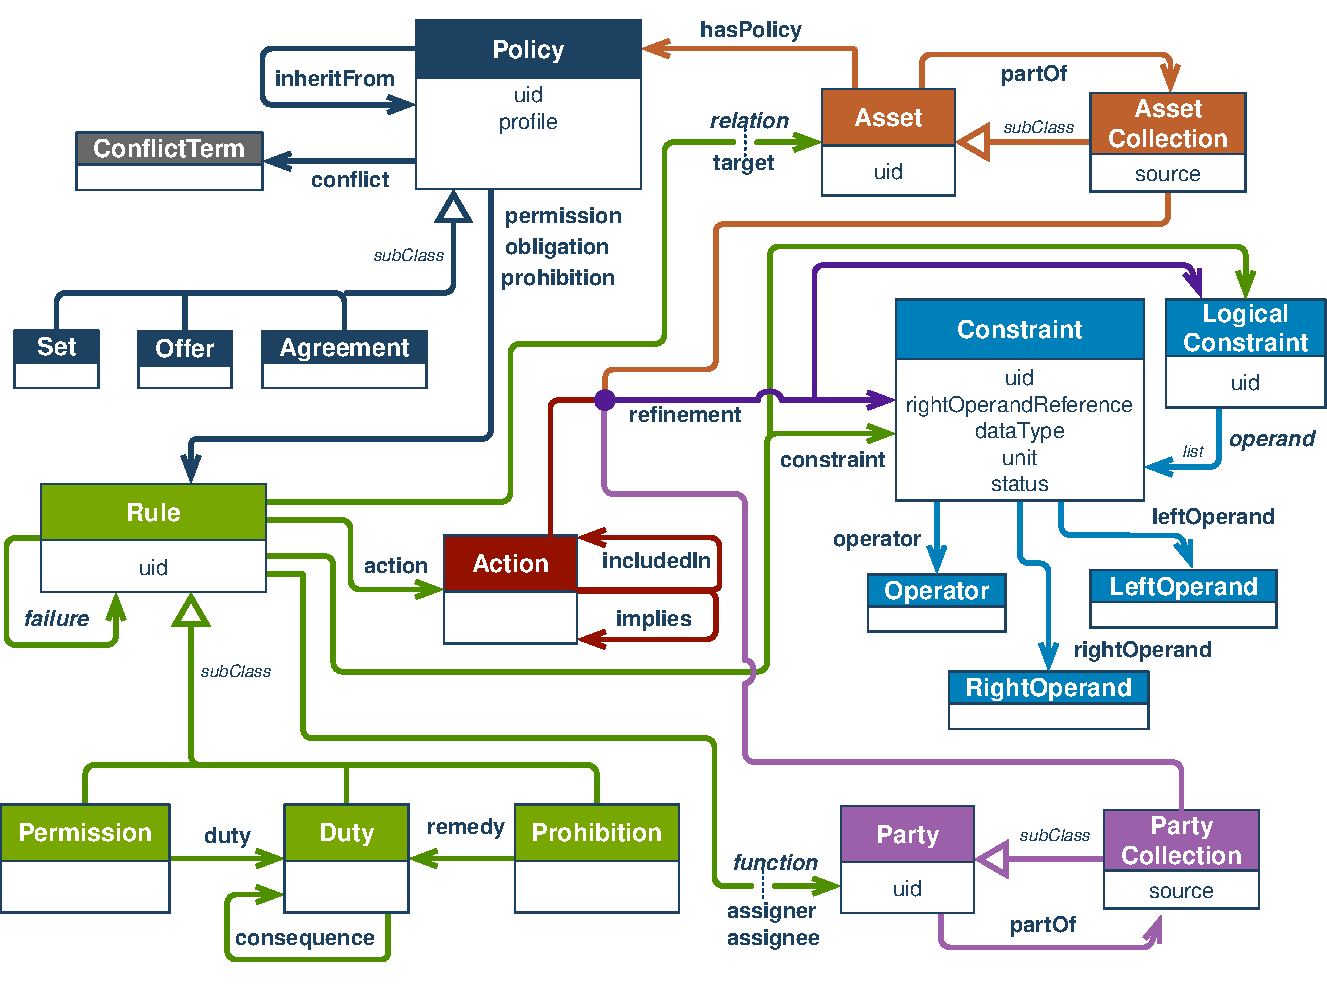
\includegraphics{ODRLModel.pdf}}
	
	\caption{Schema del modello ODRL\cite{ODRLinfMod}\label{ODRLModelSchema}}
\end{figure}
Come visibile all'interno dello schema in figura \ref{ODRLModelSchema}, il modello è basato sulle seguenti entità principali:
\begin{itemize}
	\item \textbf{Policy}: un gruppo di una o più regole;
	\item \textbf{Regola}: concetto astratto che racchiude le caratteristiche comuni di \textbf{permesso}, \textbf{divieto}, \textbf{doveri};
	\item \textbf{Asset}: risorsa o collezione di risorse soggette a regole;
	\item \textbf{Azione}: operazione su un asset;
	\item \textbf{Party}: entità o insieme di entità con un certo ruolo in una regola;
	\item \textbf{Limiti}: espressione logica o booleana imposta su azioni, party, asset o regole.
\end{itemize}
\paragraph{Vocabolari}\mbox{}\\
\label{profili}
``L' \textit{ODRL Vocabulary and Expression} descrive i termini usati dalle policy ODRL e come codificarle''\cite{ODRVocab}. All'interno di ODRL, i vocabolari utilizzati per definire i termini all'interno delle policy vengono detti \textbf{profili}, i quali possono essere usati per definire termini che supportano specifiche applicazioni; all'interno di un profilo è possibile, ad esempio, fornire le specifiche riguardanti nuove sottoclassi di termini già presenti nei vocabolari standard di ODRL. I 2 vocabolari principali definiti sono:
\begin{itemize}
	\item \textbf{ODRL Core Vocabulary}: rappresenta la minima espressione di policy supportata;
	\item \textbf{ODRL Common Vocabulary}: arricchisce il vocabolario precedente con un gruppo di azioni generiche, nuove sottoclassi per le policy, ruoli per i party e relazioni tra gli asset.
\end{itemize}
Una delle principali differenze tra i due vocabolari, la si ha all'interno delle \textbf{azioni} che possono essere indicate: nel primo caso si hanno a disposizione solamente 2 azioni \textbf{use} e \textbf{transfer}, nel secondo caso queste 2 azioni vengono estese da diverse azioni figlie, come mostrato in figura \ref{imgUseTransfer}

\begin{figure}[H]
	\centering
	\def\svgwidth{\columnwidth}
	\scalebox{0.35}{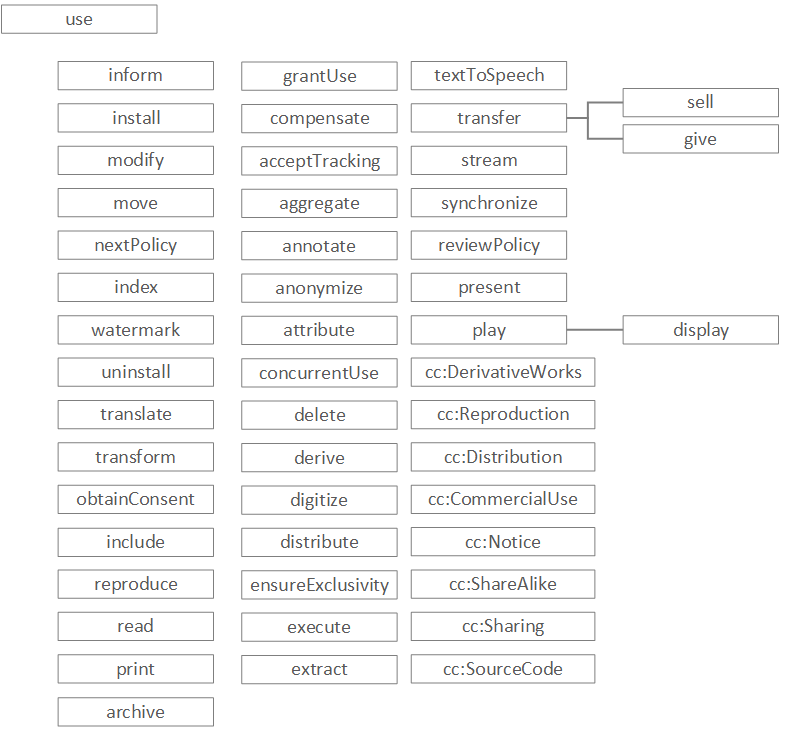
\includegraphics{useTree.png}}
	
	\caption{Tutte le azioni mostrate sono figlie di use, ad eccezioni di trasfer e le sue sottoazioni\cite{ODRLBestPract}\label{imgUseTransfer}}
\end{figure}


\paragraph{Policy}\mbox{}\\
Come definito nel modello presente nella sezione \ref{modello}, una policy è un gruppo non vuoto di \textbf{regole} e, quindi, di \textbf{permessi}, \textbf{divieti} o \textbf{obblighi}. Una policy deve soddisfare i seguenti requisiti:
\begin{itemize}
	\item deve avere un identificativo univoco, detto \textbf{uid};
	\item deve avere almeno una regola;
	\item può specificare un profilo, obbligatorio se non si usa il Core Vocabulary mostrato nella sezione \ref{profili};
	\item può specificare una policy da cui eredita le proprietà;
	\item può specificare una strategia per la risoluzione dei conflitti.
\end{itemize}
Come visibile dalla figura \ref{ODRLModelSchema}, una policy ha 3 prossibili sottoclassi:
\begin{itemize}
	\item \textbf{Set}: un insieme di regole che hanno effetto;
	\item \textbf{Agreement}: regole concesse ad una entità assegnataria da una assegnatrice;
	\item \textbf{Offer}: proposta di una regola da parte di un assegnatore.
\end{itemize}
Di seguito un esempio di policy definita mediante ODRL:
\begin{lstlisting}[language=json,firstnumber=1,caption={Policy con sottoclasse \textbf{Set}},captionpos=b,label=esmpioPolicy]
{
 "@context": "http://www.w3.org/ns/odrl.jsonld",
 "@type": "Set",
 "uid": "http://example.com/policy:1010",
 "permission": [{
   "target": "http://example.com/asset:9898.movie",
   "action": "use"
 }]
}
\end{lstlisting}
La policy mostrata nel listing \ref{esmpioPolicy} presenta i campi:
\begin{itemize}
	\item @type: serve ad indicarne la sottoclasse;
	\item @context : serve ad indicare che il file deve essere conforme ad ODRL, rappresentato dall'URL da cui si può ottenere l'ODRL Common Vocabulary\cite{ODRLCV};
	\item nel contesto sono presenti altri link per le altre proprietà, ad esempio quello per la descrizione di \textit{Set} e per \textit{use};
	\item non usando termini fuori dai 2 vocabolari principali, non necessita la definizione di un profilo;
	\item l'id univoco è rappresentato da un URL che porta alle informazioni relative la risorsa.
\end{itemize}
\paragraph{Asset}\mbox{}\\
Come definito nel modello presente nella sezione \ref{modello}, un asset è una risorsa o una collezione di risorse soggette a regole. Un asset può essere una qualunque risorsa identificabile. Ha \textbf{AssetCollection} come sottoclasse, la quale rappresenta una collezione di asset. La classe asset può avere:
\begin{itemize}
\item un identificativo univoco, il quale può essere omesso se l'asset è fornito direttamente con la policy; le specifiche di ODRL, pur supportando questo caso d'uso, sconsigliano questa pratica;
\item una o più proprietà denominate \textbf{partOf}: identifica le collezioni di cui fa parte l'asset, il quale può essere a sua volta una collezione.
\end{itemize}
Esempio di utilizzo in una regola:
\begin{lstlisting}[language=json,firstnumber=1,caption={Utilizzo di asset nella proprietà \textbf{target} di una regola},captionpos=b,label=esempioAsset]
{
"@context": "http://www.w3.org/ns/odrl.jsonld",
 "@type": "Offer",
 "uid": "http://example.com/policy:3333",
 "profile": "http://example.com/odrl:profile:02",
 "permission": [{
	"target": "http://example.com/asset:3333",
	"action": "display",
	"assigner": "http://example.com/party:0001"
 }]
}
\end{lstlisting}
La sottoclasse \textbf{AssetCollection} può avere i seguenti 2 campi aggiuntivi:
\begin{itemize}
	\item \textbf{source}: sostituisce il campo \textbf{uid} nelle classe AssetCollection all'interno di un \textbf{refinement};
	\item una o più \textbf{refinement}: limiti riguardanti la collezione che identificano solamente un sottogruppo di asset al suo interno.
\end{itemize}
Esempio di utilizzo della proprietà \textbf{partOf}:
\begin{lstlisting}[language=json,firstnumber=1,caption={L'asset definito è parte del target presente nel listing \ref{esempioAsset}},captionpos=b,label=esempioAssetColl]
{
	"@type": "dc:Document",
	"@id": "http://example.com/asset:111.doc",
	"dc:title": "Annual Report",
	...
	"odrl:partOf": "http://example.com/archive1011",
	...
}
\end{lstlisting}
In quest'ultimo esempio si ha che l'asset con id ``\url{http://example.com/asset:111.doc}'' è definito come parte della collezione ``\url{http://example.com/archive1011}''. Questa definizione ha come effetto l'applicarsi della policy presente nel listing \ref{esempioAsset} anche all'asset che fa parte della collezione.
\paragraph{Party}\mbox{}\\
Come definito nel modello presente nella sezione \ref{modello}, un party è una entità o una collezione di entità con una funzione determinata in una regola. Un party può essere un qualunque soggetto con un ruolo attivo nelle regole o che produce un effetto specifico, ad esempio controlla che le azione relative ad un dovere vengano effettuate. Ha \textbf{PartyCollection} come sottoclasse, la quale rappresenta una collezione di entità. La classe party può avere:
\begin{itemize}
	\item un identificativo univoco, il quale può essere omesso se è possibile definire in altro modo l'entità; le specifiche di ODRL, pur supportando questo caso d'uso, sconsigliano questa pratica;
	\item una o più proprietà denominate \textbf{partOf}: identifica le collezioni di cui fa parte l'entità, la quale può essere a sua volta una collezione.
\end{itemize}
Esempio di utilizzo in una regola:
\begin{lstlisting}[language=json,firstnumber=1,caption={Utilizzo di party nelle proprietà \textbf{assigner} ed \textbf{assignee} di una regola},captionpos=b,label=esempioParty]
{
"@context": "http://www.w3.org/ns/odrl.jsonld",
"@type": "Agreement",
"uid": "http://example.com/policy:8888",
"profile": "http://example.com/odrl:profile:04",
"permission": [{
"target": "http://example.com/music/1999.mp3",
"assigner": "http://example.com/org/sony-music",
"assignee": "http://example.com/people/billie",
"action": "play"
}]
}  
\end{lstlisting}
La sottoclasse \textbf{PartyCollection} può avere i seguenti 2 campi aggiuntivi:
\begin{itemize}
	\item \textbf{source}: sostituisce il campo \textbf{uid} nelle classe PartyCollection all'interno di un \textbf{refinement};
	\item una o più \textbf{refinement}: limiti riguardanti la collezione che identificano solamente un sottogruppo di asset al suo interno.
\end{itemize}
Esempio di utilizzo della proprietà \textbf{partOf}:
\begin{lstlisting}[language=json,firstnumber=1,caption={L'entità definita è parte di una PartyCollection},captionpos=b,label=esempioPartyColl]
{
"@type": "vcard:Individual",
"@id": "http://example.com/person/murphy",
"vcard:fn": "Murphy",
"vcard:hasEmail": "murphy@example.com",
...
"odrl:partOf": "http://example.com/team/A",
...
}
\end{lstlisting}
In quest'ultimo esempio si ha che l'entità con id ``\url{http://example.com/person/murphy}'' è definita come parte della collezione ``\url{http://example.com/team/A}''. Questa definizione ha come effetto l'affidare le funzioni di quest'ultima collezione anche alla singola entità che ne fa parte.
\paragraph{Action}\mbox{}\\
Come definito nel modello presente nella sezione \ref{modello}, \textbf{action} è una classe che rappresenta un'operazione che può essere esercitata su un asset, al quale viene associata mediante la propietà \textbf{action} di una regola. Nell' ODRL Core Vocabulary sono presenti 2 azioni principali:
\begin{itemize}
	\item use: un qualsiasi utilizzo dell'asset;
	\item transfer: una qualsiasi azione che preveda il trasferimento di proprietà dell'asset;
\end{itemize}
Un'azione può avere le seguenti proprietà:
\begin{itemize}
	\item refinement: raffinamenti semantici sull'azione, come ad esempio l'ammontare di un pagamento, il luogo nel quale l'azione può essere eseguita o il tempo massimo di esecuzione;
	\item includedIn: esprime l'azione padre; la conseguenza di questa dichiarazione risulta essere che tutte le regole applicate all'azione padre, devono valere anche per l'azione figlia;
	\item implies: esprime un'azione che non deve essere vietata per permettere l'azione con questa proprietà, ma le 2 azioni non hanno una relazione espressa tramite \textit{includedIn}\footnote{attualmente né l'ODRL Core Vocabulary né l'ODRL Common Vocabulary presentano azioni con questa proprietà}. 
\end{itemize}
Come anticipato nel paragrafo \ref{profili} relativo ai profili, l'ORDL Common Vocabulary utilizza la proprietà \textit{includedIn} per aggiungere azioni figlie sia ad \textit{use} che \textit{transfer}, come già mostrato nella figura \ref{imgUseTransfer}.\\
Di seguito un esempio di azione in una regola:
\begin{lstlisting}[language=json,firstnumber=1,caption={L'azione \textbf{play} è presente nella proprietà \textbf{action} della regola},captionpos=b,label=esempioAction]

{
	"@context": "http://www.w3.org/ns/odrl.jsonld",
	"@type": "Offer",
	"uid": "http://example.com/policy:1012",
	"profile": "http://example.com/odrl:profile:06",
	"permission": [{
		"target": "http://example.com/music:1012",
		"assigner": "http://example.com/org:abc",
		"action": "play"
	}]
}
\end{lstlisting}
\paragraph{Constraint e Logical Constraint}\mbox{}\\
Come definito nel modello presente nella sezione \ref{modello}, \textbf{constraint} è una classe usata per comparare 2 espressioni che non sono constraint a loro volta, utilizzando un operatore relazionale. Rappresentano una limitazione tramite un confronto, la quale può essere soddisfatta o non soddisfatta. La classe presenta le seguenti proprietà:
\begin{itemize}
	\item uno o nessun identificativo univoco, qualora si volesse riutilizzare l'espressione di confronto definita;
	\item un \textbf{leftOperand}: elemento a sinistra dell'operatore di confronto;
	\item un sottotitpo \textbf{operator}: operatore di confronto;
	\item uno tra: 
	\begin{itemize}
		\item \textbf{rightOperand}: elemento a destra dell'operatore di confronto, identificato direttamente;
		\item \textbf{rightOperand}: elemento a destra dell'operatore di confronto, identificato con un riferimento; 
	\end{itemize} 
	\item uno o nessun \textbf{dataType}: definisce il tipo dell'operando di destra;
	\item una o nessuna \textbf{unit}: unità di misura dell'operando di destra;
	\item uno o nessun \textbf{status}: per l'elemento di sinistra.
\end{itemize}
Oltre ai normali constraint, il modello definisce anche dei logical constraint, ovvero operazioni logiche su altri constraint già definiti. In questo caso le proprietà sono:
\begin{itemize}
	\item uno o nessun identificativo univoco, qualora si volesse riutilizzare l'espressione di confronto definita;
	\item un sottotipo di \textbf{operand}: operatore logico tra i constraint espressi come lista al suo interno.
\end{itemize}
Esempi di utilizzi dei constraint: 
\begin{lstlisting}[language=json,firstnumber=1,caption={Constraint su azione: l'azione \textbf{print} è permessa solo per risoluzioni minori di 1200 dpi},captionpos=b,label=esempioRef]
{
 "@context": "http://www.w3.org/ns/odrl.jsonld",
 "@type": "Offer",
 "uid": "http://example.com/policy:6161",
 "profile": "http://example.com/odrl:profile:10",
 "permission": [{
  "target": "http://example.com/document:1234",
   "assigner": "http://example.com/org:616",
   "action": [{
  	"rdf:value": { "@id": "odrl:print" },
  	"refinement": [{
  		"leftOperand": "resolution",
  		"operator": "lteq",
  		"rightOperand": { "@value": "1200", "@type": "xsd:integer" },
  		"unit": "http://dbpedia.org/resource/Dots_per_inch"
    	}]
 	}]
  }]
}
\end{lstlisting}
\begin{lstlisting}[language=json,firstnumber=1,caption={Constraint logico su azione: l'azione \textbf{reproduce} è permessa solo nella forma di uno dei due constraint listati},captionpos=b,label=esempioLogRef]
{
 "@context": "http://www.w3.org/ns/odrl.jsonld",
 "@type": "Offer",
 "uid": "http://example.com/policy:88",
 "profile": "http://example.com/odrl:profile:10",
 "permission": [{
  "target": "http://example.com/book/1999",
  "assigner": "http://example.com/org/paisley-park",
  "action": [{
    "rdf:value": { "@id": "odrl:reproduce" },
	"refinement": {
	  "xone": { 
	    "@list": [ 
		 { "@id": "http://example.com/p:88/C1" },
		 { "@id": "http://example.com/p:88/C2" } 
		]}
	}
  }]
 }]
}
\end{lstlisting}
\begin{lstlisting}[language=json,firstnumber=1,caption={Constraint su asset: l'azione \textbf{play} è permessa solo sui target di durata strettamente inferiore a 60 minuti},captionpos=b,label=esempioConAss]
{
"@context": "http://www.w3.org/ns/odrl.jsonld",
"@type": "Offer",
"uid": "http://example.com/policy:4444",
"profile": "http://example.com/odrl:profile:11",
"permission": [{
 "assigner": "http://example.com/org88",
 "target": {
 	"@type": "AssetCollection",
 	"source":  "http://example.com/media-catalogue",
 	"refinement": [{
 		"leftOperand": "runningTime",
 		"operator": "lt",
 		"rightOperand": { 
 		 "@value": "60",
 		 "@type": "xsd:integer"
 		 },
 		"unit": "http://qudt.org/vocab/unit/MinuteTime"
 	}]
 },
 "action": "play"
}]
}
\end{lstlisting}
\begin{lstlisting}[language=json,firstnumber=1,caption={Constraint su party: l'azione \textbf{view} è permessa solo alle entità con età strettamente superiore a 17 anni},captionpos=b,label=esempioConParty]
{
"@context": "http://www.w3.org/ns/odrl.jsonld",
"@type": "Agreement",
"uid": "http://example.com/policy:4444",
"profile": "http://example.com/odrl:profile:12",
"permission": [{
  "target": "http://example.com/myPhotos:BdayParty",
  "assigner": "http://example.com/user44",
  "assignee": {
     "@type": "PartyCollection",
 	 "source":  "http://example.com/user44/friends",
 	 "refinement": [{
 	 	"leftOperand": "foaf:age",
 	 	"operator": "gt",
 	 	"rightOperand": { 
 	 	 "@value": "17",
 	 	 "@type": "xsd:integer"
 		 }
 	 }]
 	},
  "action": { "@id": "ex:view" }
}]
}
\end{lstlisting}
\paragraph{Rule}\mbox{}\\
Come definito nel modello presente nella sezione \ref{modello}, \textbf{rule} è una classe astratta che raccoglie gli aspetti comuni della classi  \textbf{permission}, \textbf{prohibition}, and \textbf{duty}. Rappresenta una delle regole all'interno della policy. Presenta le seguenti proprietà:
\begin{itemize}
	\item una \textbf{action}: azione regolamentata;
	\item una o nessuna \textbf{relation}: asset sul quale si applica la regola;
	\item una, nessuna o più \textbf{function}: funzioni che un party può avere all'interno di una regola;
	\item uno, nessuno o più \textbf{constraint }: limiti applicati alla validità della regola;
	\item uno o nessun identificativo univoco, necessario solo qualora si usare la regola per ereditarne le proprietà;
\end{itemize}
Le sottoclassi sono così definite:
\begin{itemize}
	\item \textbf{permission}: permette un'azione sull'asset specificato, con tutti i \textbf{refinement} di quest'ultima soddisfatti; inoltre l'azione può essere eseguita solo se tutti i limiti della regola sono soddisfatti e ogni dovere espresso come \textbf{duty} è stato rispettato. Un permesso rende obbligatoria la \textbf{relation} denominata \textbf{target};
	\item \textbf{prohibition}: vieta un'azione sull'asset specificato, con tutti i \textbf{refinement} di quest'ultima soddisfatti; inoltre l'azione non può essere eseguita solo se tutti i limiti della regola sono soddisfatti; se si infrange il divieto, ogni dovere espresso come \textbf{remedy} deve essere eseguito. Un divieto rende obbligatoria la \textbf{relation} denominata \textbf{target};
	\item \textbf{duty}: obbligo di eseguire un'azione, con tutti i \textbf{refinement} di quest'ultima soddisfatti; un dovere è compiuto se tutti i suoi limiti sono soddisfatti e la sua azione effettuata, con tutti i \textbf{refinement} definiti. Se un dovere non è stato compiuto, bisogna eseguirne le \textbf{consequences}, ovvero altri doveri da compiere.
\end{itemize}
Esempi di regole all'interno di policy:
\begin{lstlisting}[language=json,firstnumber=1,caption={La regola esprime il permesso di eseguire l'azione \textbf{play} sul target fino al giorno 2017-12-31 compreso},captionpos=b,label=esempioPerm]
{
 "@context": "http://www.w3.org/ns/odrl.jsonld",
 "@type": "Offer",
 "uid": "http://example.com/policy:9090",
 "profile": "http://example.com/odrl:profile:07",
 "permission": [{
    "target": "http://example.com/game:9090",
    "assigner": "http://example.com/org:xyz",
    "action": "play",
    "constraint": [{
        "leftOperand": "dateTime",
        "operator": "lteq",
        "rightOperand": { "@value": "2017-12-31", "@type": "xsd:date" }
    }]
  }]
}
\end{lstlisting}
\begin{lstlisting}[language=json,firstnumber=1,caption={La regola esprime il divieto di eseguire l'azione \textbf{archive} sul target},captionpos=b,label=esempioPro]
{
 "@context": "http://www.w3.org/ns/odrl.jsonld",
 "@type": "Agreement",
 "uid": "http://example.com/policy:5555",
 "profile": "http://example.com/odrl:profile:08",
 "prohibition": [{
	"target": "http://example.com/photoAlbum:55",
	"action": "archive",
	"assigner": "http://example.com/MyPix:55",
	"assignee": "http://example.com/assignee:55"
 }]
}
\end{lstlisting}

\begin{lstlisting}[language=json,firstnumber=1,caption={La regola esprime l'obbligo di eseguire l'azione \textbf{compensate}, specificando come \textbf{refinement} l'ammontare del pagamento},captionpos=b,label=esempioDuty]
{
"@context": "http://www.w3.org/ns/odrl.jsonld",
"@type": "Agreement",
"uid": "http://example.com/policy:42",
"profile": "http://example.com/odrl:profile:09",
"obligation": [{
 "assigner": "http://example.com/org:43",
 "assignee": "http://example.com/person:44",
 "action": [{
   "rdf:value": {
     "@id": "odrl:compensate"
   },
   "refinement": [
     {
     "leftOperand": "payAmount",
     "operator": "eq",
     "rightOperand": { "@value": "500.00", "@type": "xsd:decimal" },
     "unit": "http://dbpedia.org/resource/Euro"
   }]
  }]
 }]
}
\end{lstlisting}
\bibliography{cit}{}
\bibliographystyle{plain}
\end{document}